% Created 2024-01-20 Cts 22:26
% Intended LaTeX compiler: pdflatex
\documentclass[presentation,smaller]{beamer}
\usepackage[utf8]{inputenc}
\usepackage[T1]{fontenc}
\usepackage{graphicx}
\usepackage{longtable}
\usepackage{wrapfig}
\usepackage{rotating}
\usepackage[normalem]{ulem}
\usepackage{amsmath}
\usepackage{amssymb}
\usepackage{capt-of}
\usepackage{hyperref}
\usetheme{Copenhagen}
\author{Eren Hatırnaz}
\date{20 Ocak 2024}
\title{Emacs 101: Yeni başlayanlar için Emacs}
\subtitle[INST]{Cumartesi Buluşması \#3 \\ Samsun Developers}
\hypersetup{
 pdfauthor={Eren Hatırnaz},
 pdftitle={Emacs 101: Yeni başlayanlar için Emacs},
 pdfkeywords={},
 pdfsubject={},
 pdfcreator={Emacs 29.1 (Org mode 9.6.6)}, 
 pdflang={Turkish}}
\begin{document}

\maketitle
\begin{frame}{Outline}
\tableofcontents
\end{frame}


\section{Ben Kimim}
\label{sec:orgc35fbde}
\begin{frame}[label={sec:orgfb7ecbb}]{Eren Hatırnaz}
\begin{center}

\includegraphics[height=2.3cm]{../_images/profile_photo.jpg}
\end{center}
\begin{itemize}
\item Technical Product Owner @ \href{https://mobillium.com}{Mobillium} (ex Back-End Developer)
\item GNU/Linux Geek
\item \href{https://instagram.com/erenhatirnaz}{Hobbyist Photographer}
\item Twitter: \href{https://twitter.com/erenhatirnaz}{@erenhatirnaz}
\item \href{https://erenhatirnaz.com}{erenhatirnaz.com} • \href{mailto:eren@hatirnaz.com.tr}{eren@hatirnaz.com.tr}
\end{itemize}
\end{frame}
\section{Emacs nedir?}
\label{sec:org4009acc}
\begin{frame}[label={sec:orgd3539ee}]{Emacs hakkında}
\begin{center}

\includegraphics[height=2cm]{./_images/emacs_logo.png}
\end{center}

\begin{itemize}
\item Emacs aslında bir text editörden çok daha fazlası\ldots{} aslında bir "programlama ortamı"!
\item İlk olarak 70'li yıllarda MIT laboratuvarlarında geliştirilmeye başlanıyor.
\item Günümüzde en çok kullanılan GNU Emacs ise 1984 yılında Richard Stallman
tarafından geliştirilmeye başlanıyor. Bugün ise GNU projesinin bir parçasıdır.
\item Extensible, Self-documented, Accessible ve en önemlisi Özgür Yazılım
\end{itemize}
\end{frame}
\begin{frame}[label={sec:org5fb5876}]{Lisp, CommonLisp, EmacsLisp\ldots{}}
\begin{itemize}
\item Lisp, fonksiyonal paradigmaya sahip bir programlama dilidir.
\item Lehçeleri:
\begin{itemize}
\item CommonLisp
\item EmacsLisp
\item AutoLisp
\item Clojure
\item \ldots{}
\end{itemize}
\end{itemize}
\end{frame}
\begin{frame}[label={sec:orgf782eea},fragile]{EmacsLisp örnekleri}
 \begin{block}{Örnek 1}
\begin{verbatim}
(defun sum (num1 num2)
  (+ num1 num2))

(sum 4 5)
\end{verbatim}
\end{block}

\begin{block}{Örnek 2}
\begin{verbatim}
(defun is-even-or-odd (num1)
  (if (= (% num1 2) 0)
      (message-box (format "%d cift sayidir" num1))
    (message-box (format "%d tek sayidir" num1))))

(is-even-or-odd 2)
\end{verbatim}
\end{block}
\end{frame}
\begin{frame}[label={sec:org91351a9}]{:))}
\begin{center}
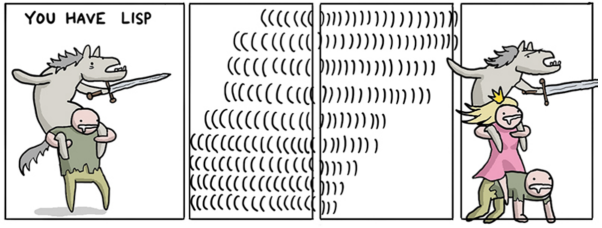
\includegraphics[width=.9\linewidth]{./_images/lisp_meme.png}
\end{center}

\begin{center}
\href{https://res.cloudinary.com/aas-sh/image/upload/v1617292960/blog/2019/07/languages\_meme\_full\_f54fux.jpg}{Kaynak}
\end{center}
\end{frame}
\begin{frame}[label={sec:org9640c41}]{Learning Curve}
\begin{center}
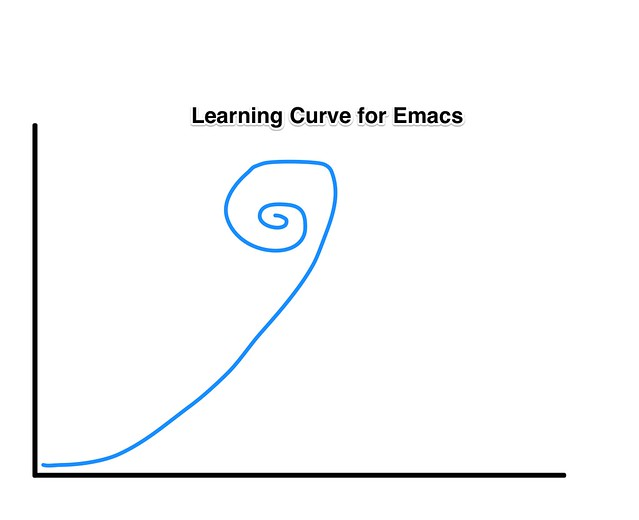
\includegraphics[height=5cm]{./_images/emacs_learning_curve.jpg}
\end{center}

\begin{center}
"Emacs has a never-ending learning curve"*

*\url{https://chadstovern.com/emacs-is-a-way-of-life/}
\end{center}
\end{frame}
\section{Temel Kavramlar}
\label{sec:org1c3fa60}
\begin{frame}[label={sec:org999c917}]{Frame \& Window \& Buffer}
\begin{itemize}
\item \alert{Frame}: Emacs penceresinin tümüne verilen isim.
\item \alert{Window}: Emacs penceresinin içerisindeki bölmelere verilen isim.
\item \alert{Buffer}: Düzenleme ve metin işleme işlemleri için kullanılan temel kavramlardan biridir.
\begin{itemize}
\item Temp (Geçici) Buffer
\item File (Dosya) Buffer
\end{itemize}
\end{itemize}
\end{frame}
\begin{frame}[label={sec:orgb5b1869},fragile]{Keybindings}
 \begin{itemize}
\item En temel iki kısayolumuz var: \texttt{C-x} ve \texttt{M-x}
\item Meta = Alt = Command
\item Cursor hareketleri
\item Tekrarlanabilirlik \texttt{C-u}
\item \texttt{kill} ve \texttt{yank} kavramlar (cut \& paste)
\end{itemize}
\end{frame}
\begin{frame}[label={sec:orgee5d1bd}]{Major Mode \& Minor Mode}
\begin{itemize}
\item \alert{Major Mode}: Ana düzenleme modunu temsil eder ve genellikle belirli bir görev
veya dosya türü için özel işlevselliği içerir.
\begin{itemize}
\item Aynı buffer üzerinde birden fazla major mode etkin olamaz.
\end{itemize}
\item \alert{Minor Mode}: Major modları tamamlar, ek işlevselliği sağlar ve genellikle
belirli özelliklere odaklanır.
\begin{itemize}
\item İstediğiniz kadar minor mode aktif edebilirsiniz.
\end{itemize}
\end{itemize}
\end{frame}
\begin{frame}[label={sec:org5f90eb8}]{Modeline}
\begin{itemize}
\item Modern dünyada "status bar" diye bildiğimiz kısımdır. Emacs penceresinin en
altında yer alır.
\end{itemize}
\end{frame}
\begin{frame}[label={sec:orgb9e2f87},fragile]{Macrolar}
 \begin{verbatim}
Merhaba dünya! Bu, bir örnek metindir. Hi kelimesi sıkça kullanılmaktadır.
Hi, dünyanın her yerinden insanları birleştiren evrensel bir selamlaşma
şeklidir. Hi demek, farklı kültürler arasında iletişimi kolaylaştırabilir.

Hi, sadece bir İngilizce kelime değil, aynı zamanda insanların birbirleriyle
tanışmalarına ve iletişim kurmalarına yardımcı olan güçlü bir ifadedir. Bir
topluluğun merkezi olabilir ve insanları bir araya getirebilir.

Hi, samimiyet ve karşılıklı anlayışın bir ifadesi olabilir. İnsanlar
arasındaki güçlü bağları ifade etmenin yanı sıra, yeni maceralara ve keşiflere de
kapı aralayabilir.

Hi dünyasını keşfetmek için bu metni kullanarak yukarıdaki örnek makroyu
deneyebilirsiniz. Belirli bir "hello" kelimesini seçin ve makro ile tüm "hello"
kelimelerini dolaşarak "hi" ile değiştirin. Bu, metni hızlı bir şekilde
düzenlemenin ve değişiklik yapmanın etkili bir yoludur.
\end{verbatim}
\end{frame}
\section{Hızlandırılmış Emacs Turu}
\label{sec:org078070c}
\begin{frame}[label={sec:orga954d0b}]{org-mode - Not defteri, Ajanda ve birçok şey}
\begin{itemize}
\item Tamamen plaintext şekilde çalışan işlevsel bir 'not defteri' eklentisi.
\item Kendi web sitesinden detaylıca inceleyebilirsiniz:
\url{https://orgmode.org/features.html}
\item Org-mode üzerine kurulu bir knowledge management system: \href{https://www.orgroam.com/}{org-roam}
\item Benim elim ayağım <3
\end{itemize}
\end{frame}
\begin{frame}[label={sec:org1883050}]{magit - Git Gui}
\begin{itemize}
\item Emacs içerisinde çalışan bir Git Gui'si diyebiliriz.
\item Command line deneyimine en yakın çözüm.
\item Elim ayağım 2 <3
\end{itemize}
\end{frame}
\begin{frame}[label={sec:org30a3e6c}]{dired - File \& Diretory Management}
\begin{itemize}
\item Emacs içerisinde yer alan bir dosya gezgini diyebiliriz.
\end{itemize}
\end{frame}
\begin{frame}[label={sec:orge063e9c}]{tetris}
\begin{itemize}
\item Çocukluğumuzun efsane oyunundan mahrum kalmıyorsunuz :)
\end{itemize}
\end{frame}
\begin{frame}[label={sec:org7acbf48}]{mu4e - Email Client}
\begin{itemize}
\item Emacs içerisinden e-maillerinizi yönetmenize olanak sağlayan bir paket.
\end{itemize}
\end{frame}
\begin{frame}[label={sec:org4a561c4}]{eww - Web Browser}
\begin{itemize}
\item Emacs içerisindeki ilkel bir web tarayıcı.
\end{itemize}
\end{frame}
\begin{frame}[label={sec:org7164442}]{erc - IRC Client}
\begin{itemize}
\item Emacs içerisindeki bir IRC clienti.
\end{itemize}
\end{frame}
\begin{frame}[label={sec:org9b6e3d4}]{exwm - Window Manager}
\begin{itemize}
\item Emacs'i sisteminizin window manager'ı olarak kullanmanıza olanacak sağlayan bir
paket.
\end{itemize}
\end{frame}
\begin{frame}[label={sec:org7fb694c}]{evil-mode - Vim-like mode}
\begin{itemize}
\item Vim keybinding'lerine alışkın insanlar için Emacs içerisine vim
alışkanlıklarını getiren bir paket.
\end{itemize}
\end{frame}
\section{Kapanış}
\label{sec:orgb414e60}
\begin{frame}[label={sec:orga85276a},fragile]{Kaynaklar}
 \begin{itemize}
\item Keyword \texttt{emacs start kit}
\item Farklı Emacs dağıtımları:
\begin{itemize}
\item \href{https://github.com/syl20bnr/spacemacs/tree/develop}{spacemacs}
\item \href{https://github.com/doomemacs/doomemacs}{Doom Emacs}
\end{itemize}
\item Youtube Kanalı: \url{https://www.youtube.com/@SystemCrafters}
\item Benim Emacs ayarlarım: \url{https://github.com/erenhatirnaz/dotfiles/tree/master/emacs/.emacs.d}
\end{itemize}
\end{frame}
\begin{frame}[label={sec:org8b41b54}]{Soru \& Cevap}
\begin{center}
Emacs hakkında merak ettikleriniz\ldots{}
\end{center}
\end{frame}
\begin{frame}[label={sec:orgbb57510}]{Teşekkürler!}
\begin{center}

\includegraphics[height=3cm]{../_images/repo_qrcode.png}
\end{center}

\begin{center}
\alert{\alert{Beni dinlediğiniz için teşekkür ederim!}}

\vspace{1in}

Twitter: @erenhatirnaz • eren@hatirnaz.com.tr
\end{center}
\end{frame}
\end{document}